\subsection{Критерий планарности}

\subsubsection*{Непланарность $K_5$ и $K_{3,3}$}

\begin{center}
    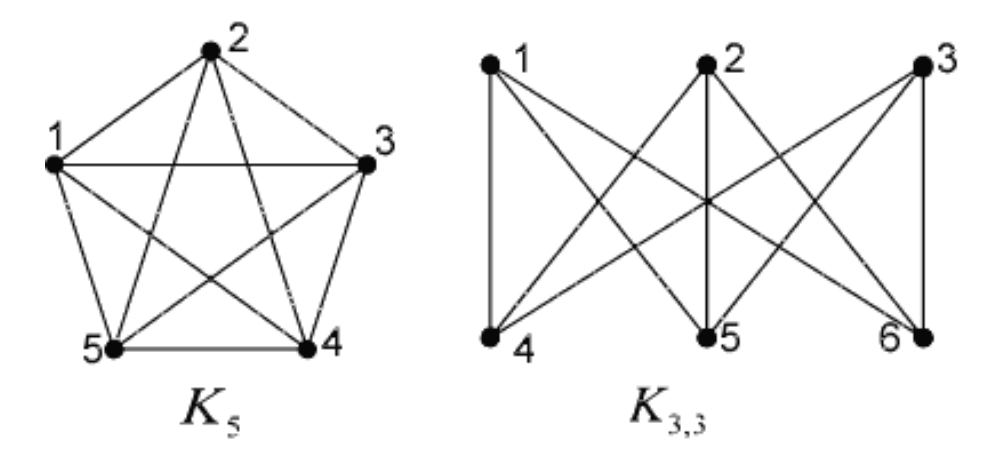
\includegraphics[width=0.4\textwidth]{par26k533.png}
\end{center}

\begin{lemma}
    Граф $K_5$ не планарен.
\end{lemma}

\begin{proof}
    В нем $|V| = 5$ и $|E| = 10$; противоречие с частью 1 теоремы \ref*{thm:3v6e}.
\end{proof}

\begin{lemma}
    Граф $K_{3,3}$ не планарен.
\end{lemma}

\begin{proof}
    В нем $|V| = 6$ и $|E| = 9$, всякий цикл имеет длину не менее чем $4$; противоречие с частью 2 теоремы \ref*{thm:3v6e}.
\end{proof}

\subsubsection*{Гомеоморфизм графов}

\begin{defn}
    Операция разбиения ребра: добавить вершину в середине ребра $(u, v) \to (u, w),~(w, v)$, где $w$ --- новая вершина.

    Графы $G_1$ и $G_2$ гомеморфны, если, применяя к каждому из них операцию разбиения ребер, можно привести их к двум изоморфным графам.
\end{defn}

\begin{theorem}[Понтрягина-Куратовского, 1930]~
    
    Граф планарен тогда и только тогда, когда он не содержит подграфов, гомеоморфных $K_5$ и $K_{3,3}$.

\end{theorem}

\begin{proof}
    
    "$\Rightarrow$":

    Пусть граф $G$ планарен, но содержит подграф $G_1$, гомеоморфный $K_5$ или $K_{3, 3}$. Тогда, имея укладку $G$, из нее извлекаем укладку $G_1$, из которой в свою очередь можно получить укладку $K_5$ или $K_{3, 3}$.

    Противоречие, так как $K_5$ и $K_{3, 3}$ не планарны.

    "$\Leftarrow$":

    Не разбираем на курсе.

\end{proof}